% #############################################################################
% This is Chapter 1
% !TEX root = ../main.tex
% #############################################################################
% Change the Name of the Chapter i the following line
\chapter{Introduction}
% The following line allows to ref this chapter
\label{chap:intro}

The continuous growth and expansion of the world population and the correspondent increase of energy needs, is one of the most relevant topics of the century. The issues caused by the increasing usage of fossil fuels and the amount of carbon dioxide produced everyday is affecting our lives and the future of the planet. In 2019, industry and buildings account for over 90\% of global electricity demand today, while transport makes up less than 2\% \cite{iea}. Recent studies show that the building sector represents 39\% and 40\% of the energy consumption and 38\% and 36\% of the CO2 emissions in the U.S. \cite{CivilUS} and Europe\cite{CivilEU}, respectively. The expansion of office buildings and the multiplication of the amount of energy needed in order to satisfy the demands of a society that is becoming more and more technologically dependent, are two catalysts for the recent increase of energy consumption. 



On the other hand, sustainable alternatives have also emerged to replace some less ecological social habits. Electric cars are the best example of this. The adoption of electric cars is a practice that has been increasing in the last decade and is expected to grow even more in the next two. Currently, the major limitation is the autonomy of the cars, since the batteries still do not have, in most cases, enough capacity to equal the autonomy performance of a fuel car. In this sense, a solution that has been adopted is the installation of charging stations in both residential and office buildings. According to \cite{charger}, the infrastructure for \ac{EV} charging is expanding and in 2019, there were about 7.3 million chargers worldwide, of which about 6.5 million were private. The power spent on charging electric cars in buildings is a new factor to be studied, both in the influence it has on the energy consumption of the building and the reduction of energy waste while using it.


The extent of available data is also multiplying, and the analysis and modeling of this data is becoming essential to minimize energy waste. Modern infrastructures are already equipped with systems capable of monitoring and controlling power usage, and there has been an increase in the number of chargers for electric cars installed in garages. The technology also evolved to allow buildings to produce their own energy. The implementation of \ac{PV} panels in buildings is an increasingly common practice. Despite the low efficiencies (from 15\% to 17\% \cite{pv}), \ac{PV} panels are becoming an important energy source for buildings, both  residential and non-residential. 









\section{Problem statement and objectives}


\ac{EDP} is a vertically integrated energy company with a consolidated position in the Iberian Peninsula, both in terms of electricity generation, distribution and supply. The energy consumption of \ac{EDP}'s Lisbon building can be divided into two categories, controlled and uncontrolled consumption. Within the category of uncontrolled consumption, some factors are identified such as the \ac{HVAC} system, lighting, among others. These factors are said to be uncontrolled, as they generally depend directly on factors such as the outside temperature and the occupancy rate of the building, respectively, variables that cannot be controlled. When it comes to controlled consumption, in the building's parking garage there is an electric car charging system for employees, denominated \ac{EVCS}. 

The main functionality of this system is to manage the charging of all the \ac{EV}s connected to the \ac{EVCSs}. This system is able to assign exactly the amount of power supplied to each vehicle, and is able to prioritize the charging, for example, a vehicle that already has 80$\%$ of battery capacity, has less priority than a discharged vehicle that has been recently connected to the grid. The system can also manage the charging procedure based on the instantaneous available power of the building, providing more capacity when there is less overall consumption, and reducing the capacity otherwise. The decision making ability of the \ac{EVCS} makes the charging of \ac{EV}s a controlled consumption process. When it comes to production, unlike generality, the building is equipped with 70 kWp (kilowatt "peak") of solar generation, which means it also has the capacity to generate power. 



Although this system is already implemented and has access to instant information about the building, the \ac{EVCS} does not have the capacity to compute a projection of production and consumption behaviour of the building in the near future. In other words, the problem this thesis aims to solve is \ac{EVCS}'s inability to identify the energy it will have available in the future to charge \ac{EV}s. This capacity would bring numerous advantages, since the knowledge of the future available power to use would allow the optimization of the electric vehicle charging procedure.

%, thus saving energy.

Taking into consideration all the listed factors, the work developed in this thesis contributes directly to minimize the unnecessary power consumption, thus contributing to a more sustainable building. At a global scale, the objective is to assist \ac{EVCS} in the handling of power utilization in the  \ac{EV}'s charging procedure. The system has access to current data, namely the total power available at each instant, but it would be useful to obtain a forecast of the power available in the near future. The knowledge of this value would bring enormous advantages, positively impacting the way \ac{EV} charging is managed. The question then arises: "How can one forecast the power available in a near future, in order to optimize the \ac{EVCS}?". The answer to this question is to create a computing architecture capable of predicting the energy available in the future, and using that forecast to feed the \ac{EVCS}. Specifically, the goal is to define a short-term power availability forecast system to help the \ac{EVCS} to manage power supply for \ac{EVCSs}. 





\section{Thesis outcome}

In the course of this dissertation, a predictive model based on \ac{ML} methodologies was developed, namely using \ac{ANNs}, capable of producing forecasts for the available power with a time target of 5, 10 and 15 minutes in the future, for a building that presents two peculiarities: it has \ac{PV} panels for energy production, and it is equipped with an electric car charging system in its parking garage. In Figure \ref{building}, the reader can observe a schematization of all the work developed during this thesis. 

\begin{figure}[h!]
    \centering
    \begin{center}
    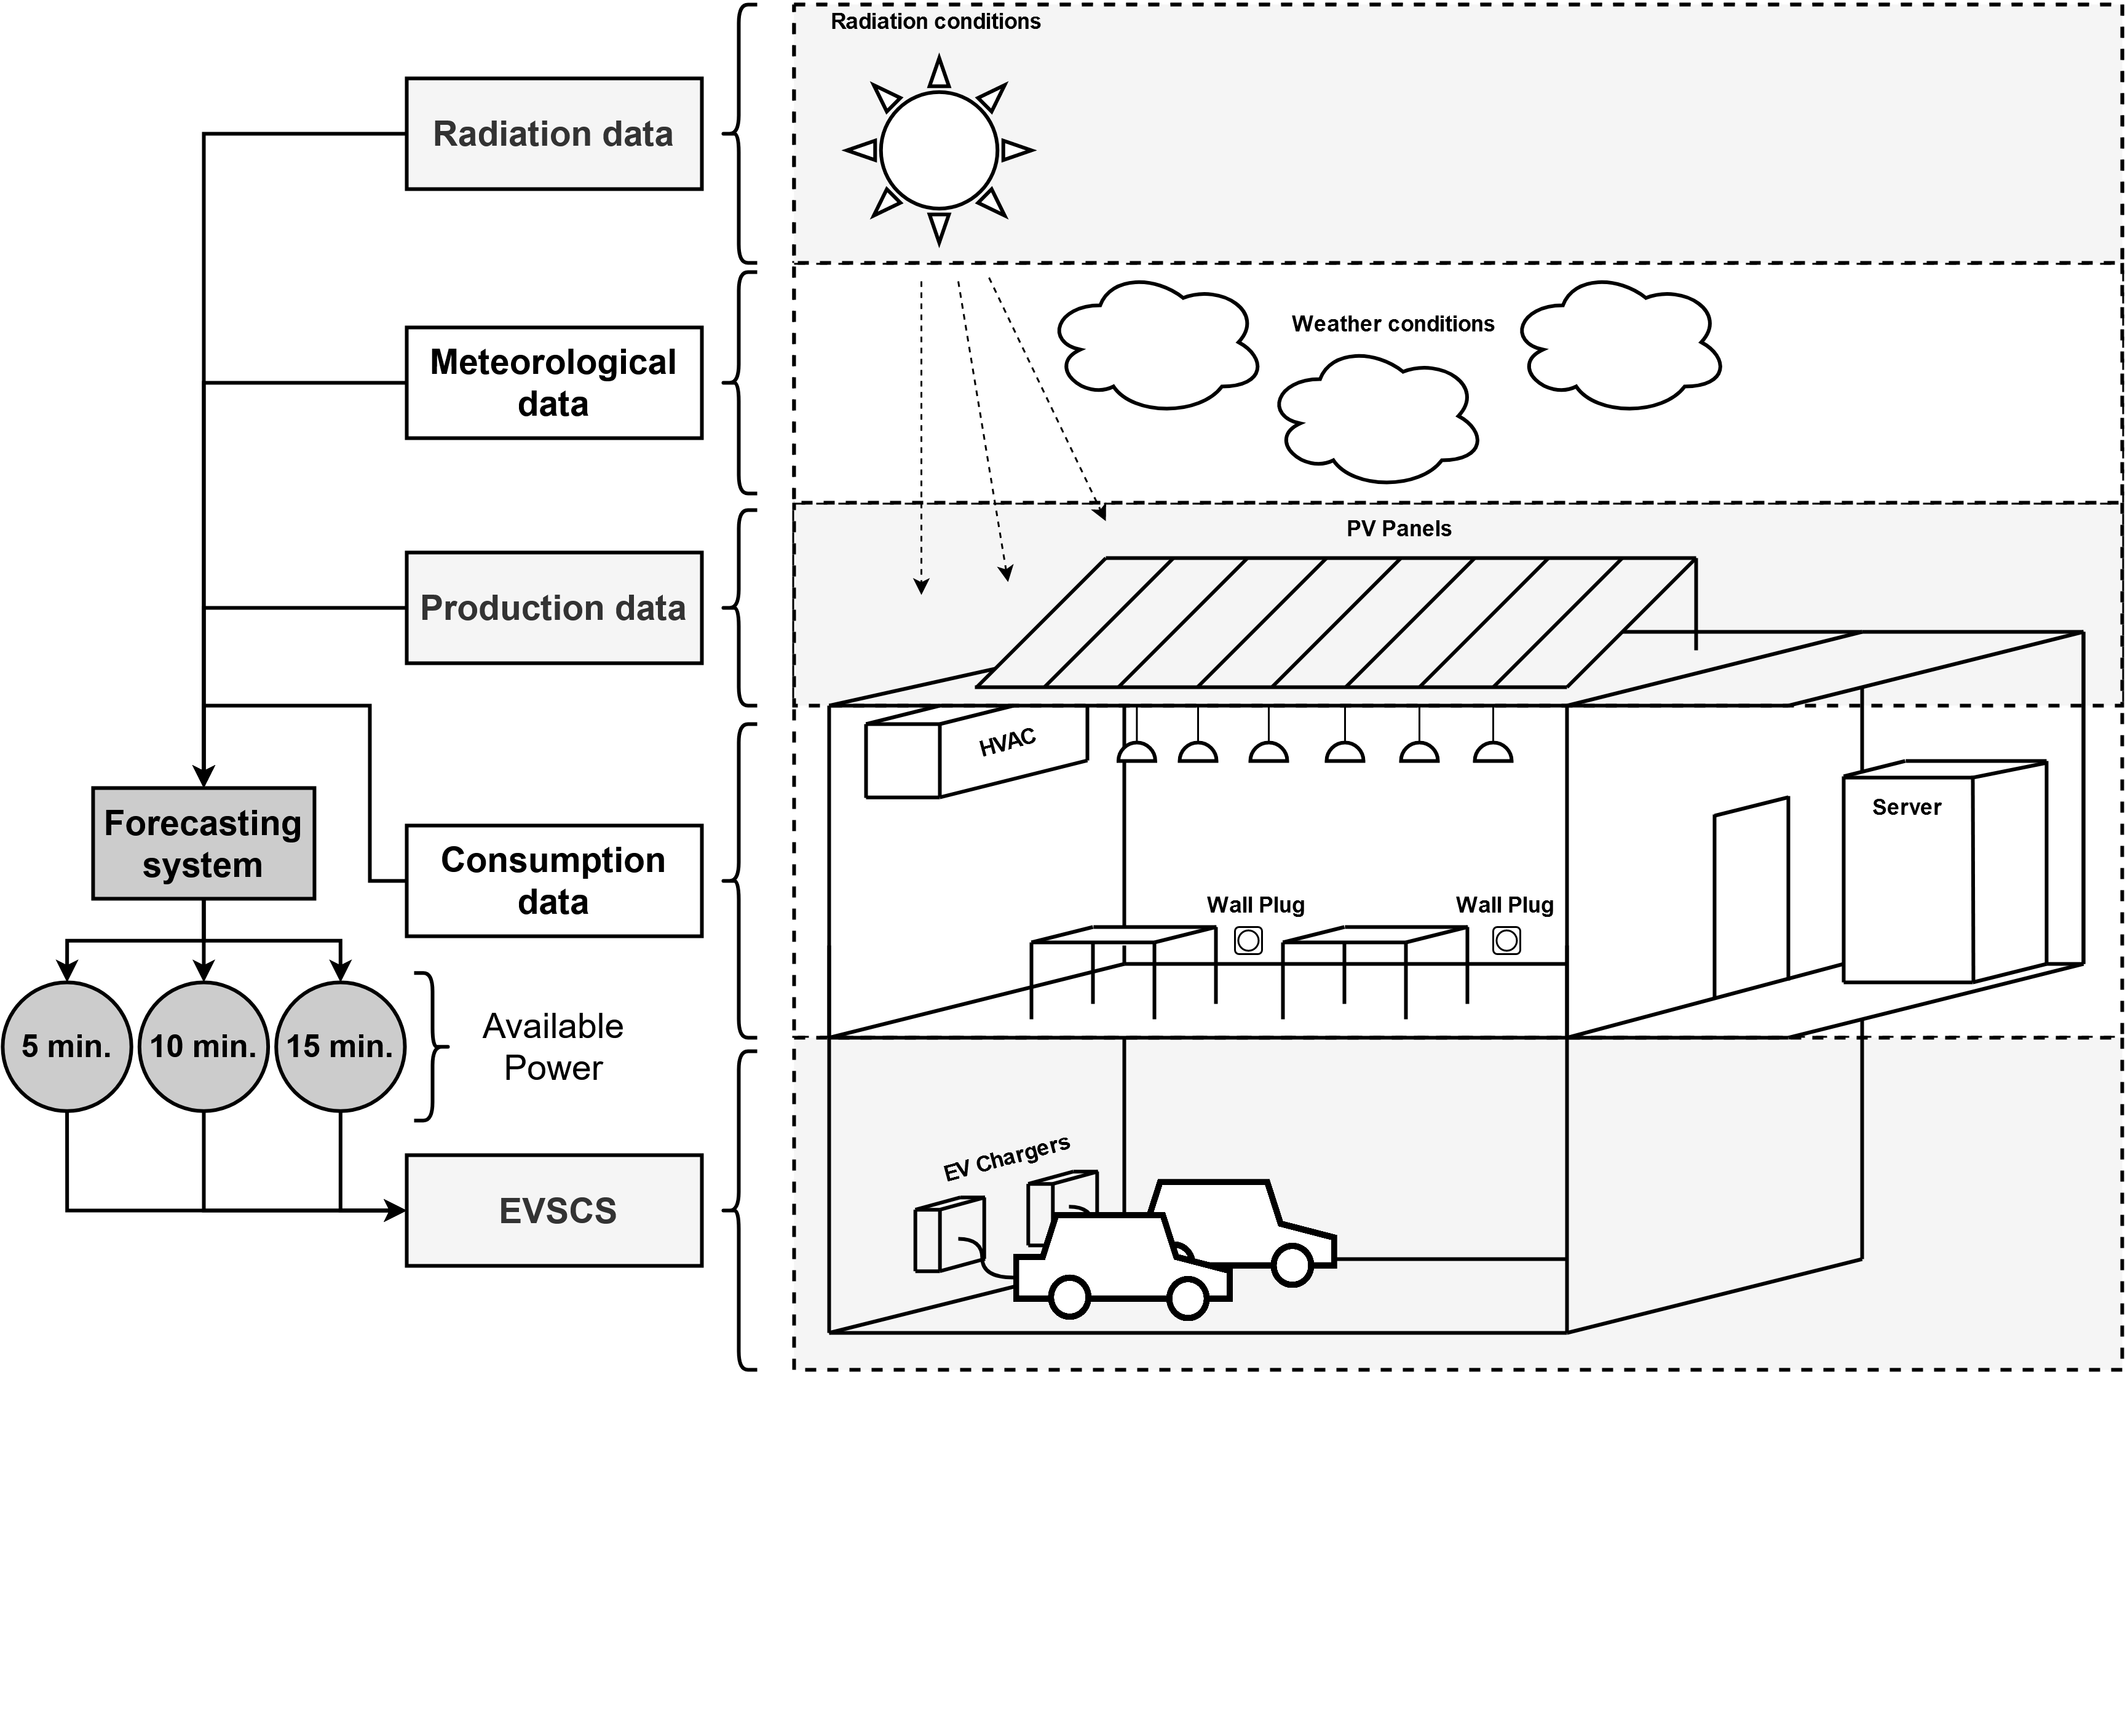
\includegraphics[width=1\textwidth]{Images/BUILDING.png}
    \caption{Building diagram.}
    \label{building}
    \end{center}
\end{figure}


A total of four datesets were used, with information on solar radiation and weather conditions of the area where the building is located, provided by \ac{FCUL}, and information regarding the power consumption and power production of the building, provided by \ac{EDP}. These datasets, besides having different dimensions and granularities, presented temporal gaps. It was then necessary to automate a data treatment process in which, regardless of the state in which the data is introduced in the system, it is treated and prepared to respect the structure that allows it to be used as input to the system. Next, six different models were developed: a Vanilla \ac{GRU}, a Vanilla \ac{LSTM}, a \ac{GRU} Encoder-Decoder, a \ac{LSTM} Encoder-Decoder, a \ac{1D CNN} - \ac{GRU} Encoder-Decoder and a \ac{1D CNN} - \ac{LSTM} Encoder-Decoder. Each one of the architectures has been built to, based on past available data, perform a forecast of the power available in the building in 5, 10 and 15 minutes. The performance of each of the architectures was evaluated and the best one was chosen. In addition, a variant of the already created models was tested and implemented, which consists of adding \ac{MCD} to the final models. The use of this methodology has the main purpose of generating random predictions and interpreting them as samples from a probabilistic distribution, which can not only help in determining the uncertainty of the model and its confidence intervals, but can improve its performance as well. 

The result of this thesis is then a forecasting system capable of generating short-term forecasts of the available power of the building. The forecasts produced by the system are later provided to the \ac{EVCS}, that uses this information to optimize its decision process. The optimization process of the charging system is outside the scope of this thesis.

\section{Thesis outline}

This thesis is composed of a total of five chapters. Chapter \ref{chap:background} introduces the background and the work already developed in this field of research, both in a general aspect, where some of the most common models of \ac{ML} are detailed, and in a more specific aspect, where some of the work developed in building consumption forecasting is presented. Chapter \ref{chap:architecture} is responsible for introducing the case study proposed, and all the procedure taken into account, namely details concerning the building in question, selection of the variable to forecast, description of all the data processing carried out, description of the models proposed and implemented, environment in which the models were tested, and finally, the performance evaluation metrics applied. The results obtained are described in Chapter \ref{chap:results}. Lastly, Chapter \ref{chap:conclusion} presents the final conclusions of this work, as long as a brief description of what was accomplished.